%%%%%%%%%%%%%%%%%%%%%%%%%%%%%%%%%%%%%%%%%%%%%%%%%%%%%%%%%%%%%%%
%
% Edit your LaTeX on the left, and it gets compiled for you on 
% the right. If you give someone the link to this page, they 
% can edit at the same time. See the help menu above for more 
% info. Enjoy!
%
%%%%%%%%%%%%%%%%%%%%%%%%%%%%%%%%%%%%%%%%%%%%%%%%%%%%%%%%%%%%%%%
\documentclass[12pt]{article}

%\usepackage[T1]{fontenc}
\usepackage{pdfpages}
\usepackage[toc,page]{appendix}
\usepackage{fancyhdr}
\usepackage{graphicx}
\usepackage{amssymb}
\usepackage{epstopdf}
\usepackage{amsmath}     
\usepackage{amssymb}
\usepackage{cite}
\usepackage{multirow}
\usepackage{wrapfig}
\usepackage{subfigure}
\usepackage{todonotes}
\usepackage{listings}
\usepackage{lipsum}
\usepackage{float}
\usepackage{tikz}
\usepackage{caption}
\usetikzlibrary{shapes.geometric, arrows}
\usepackage[colorlinks=true, linkcolor=black,citecolor=black,urlcolor=blue]{hyperref}
\bibliographystyle{IEEEtran}
\DeclareGraphicsRule{.tif}{png}{.png}{`convert #1 `dirname #1`/`basename #1 .tif`.png}
\tikzstyle{intt}=[draw,text centered,minimum size=6em,text width=5.25cm,text height=0.34cm]
\tikzstyle{intl}=[draw,text centered,minimum size=2em,text width=2.75cm,text height=0.34cm]
\tikzstyle{int}=[draw,minimum size=2.5em,text centered,text width=3.5cm]
\tikzstyle{intg}=[draw,minimum size=2em,text centered,text width=6cm]
\tikzstyle{sum}=[draw,shape=circle,inner sep=2pt,text centered,node distance=3.5cm]
\tikzstyle{summ}=[drawshape=circle,inner sep=4pt,text centered,node distance=3.cm]

%---------------- Letter Paper --------------------%
% be sure to change in document class too
\textwidth = 6.5 in
\textheight = 8.6 in
\oddsidemargin = 0.0 in
\evensidemargin = 0.0 in
\topmargin = 0.0 in
\headheight = 0.0 in
\headsep = 0.2in
\parskip = 0.2in
\parindent = 0.0in


\begin{document}
\thispagestyle{empty}
\begin{center}

% \begin{figure}
% \centering
% \includegraphics[width=0.3\textwidth]{logo.jpeg}
% \end{figure}
% \vspace{10mm}
% {\scshape \large \par INDIAN INSTITUTE OF TECHNOLOGY,DELHI }

% \vspace{0.7cm} % University name
% author names and CLIDS
\vspace*{2.2cm} 
{\LARGE \textbf{\centering SUMMER INTERNSHIP REPORT}} 
%<---- Insert your project title here
% {\LARGE \textbf{\newline \newline \centering }}
\vspace{1.0cm} \\
{\LARGE Improving Reliability of Localisation and Navigation and Development of User Interface of Mobile Robot: RoboMuse 4.0\\}

\vspace{1.0cm}

\begin{minipage}{0.6\textwidth}
\begin{center}    \large
National Institute of Technology,\\
Tiruchirappalli.\\
name \\
department\\

% Your name

\end{center}
\end{minipage}
\vspace{0.5cm}

\begin{minipage}{0.6\textwidth}
\begin{center}    \large
\emph{Supervisor:}\\
Prof. S K Saha\\ % Your name
Mechanical Engineering Department\\
Indian Institute of Technology,\\
Delhi.
\end{center}
\end{minipage}
\vspace{0.5cm}

\begin{minipage}{0.6\textwidth}
\begin{center} \large
\vspace{.2 cm}
\emph{Mentor:}\\
  Deepanshu Singh\\
  Mechanical Engineering Department\\
  Indian Institute of Technology,\\
  Delhi\\
\end{center}
\end{minipage}


\end{center}

%----------------------------------------------------------------------------------------
%    Certification Page 2
%-------------------------------------------------------------
\newpage
% \begin{figure}
% \centering
% \includegraphics[width=0.3\textwidth]{logo.jpeg}
% \end{figure}
% \vspace{0.7in}
% \begin{center}
% \textbf{Indian Institute Of Technology, Delhi}
% \end{center}

\begin{minipage}{0.6\textwidth}
\begin{large}
\vspace{7cm}
Date:\\\\
S K Saha\\
Head Of Department\\
Department of Mechanical Engineering\\
\end{large}
\end{minipage}

\vspace{1.5cm}
\begin{large}
{
This is to certify that \textbf{S. Srikrishna} an undergraduate student of The National Institute Of Technology, Tiruchirappalli, Electronics and Communication Department, (Roll Number: 108116092), had taken up a project \textbf{' Improving Reliability of Localisation and Navigation and Development of User Interface of Mobile Robot: RoboMuse 4.0'} under my guidance, during the summer of 2019 as part of an internship program from May 14,2019 to July 10,2019. 
\\\\\\\\  \\\\\\ 
} 
\end{large}
\vspace{0.7in}
\qquad\qquad\qquad\qquad\qquad\qquad\qquad\qquad\qquad\qquad\qquad\qquad\qquad\qquad\qquad\qquad \textbf{(S K Saha)} 
%----------------------------------------------------------------------------------------

\cleardoublepage

%----------------------------------------------------------------------------------------
%    ABSTRACT
%----------------------------------------------------------------------------------------
\thispagestyle{empty}
\begin{abstract}
\vspace{-0.2in}
\hspace*{-0.5cm}RoboMuse is IIT Delhi\textsc{\char13}s own ingenious mobile platform series to demonstrate 24/7
working scenario, started in 2009. Over the past 8 years, RoboMuse has had 4 iterations with each one adding something unique to the design. Over all these years the
RoboMuse was built with the essential aim of being able to function without any human
interaction  i.e autonomously and a number of applications were developed to demonstrate the requirements.\\
\\
The robot is capable of navigating through its environment in the presence of static and dynamic obstacles to reach any assigned (feasible) goals. For product development, a record of dynamic specifications of the robot including its repeatability and reproducibility is necessary. Further to demonstrate the autonomous navigation a number of applications such as NavTest, Docking the robot to charge it via different means, Following way-points in a known map and recording live video in the process were developed.\\
\\
Marker based correction for odometry for better localization was achieved by using aruco markers and transforms. Mapping was done along with multiple markers embedded in it. This map when reloaded along with markers was used for odometry correction of the robot. The robot's navigation was improved by changing the trajectory planner. Also costmap artifacts were removed by selectively clearing the costmap when required. The speech recognition was improved for the robot by tuning the pocketsphinx package. Also an UI was developed for the robot for making it easy for non technical people to use the robot easily.\\
\\
The entire system was setup on the Robot Operating System framework. The main reasons  for this being re-usability of code, modularity and ease of communication between the modules. \\
\end{abstract}

%----------------------------------------------------------------------------------------
%    ACKNOWLEDGEMENTS
%---------------------------------------------------------------------------------------
%----------------------------------------------------------------------------------------
%    LIST OF CONTENTS/FIGURES/TABLES PAGES
%----------------------------------------------------------------------------------------
\newpage
\thispagestyle{empty}
\tableofcontents
\thispagestyle{empty}
\newpage
\thispagestyle{empty}
\listoffigures
\thispagestyle{empty}
\newpage
\thispagestyle{empty}
\listoftables
\thispagestyle{empty}
%----------------------------------------------------------------------------------------
%                            INTRODUCTION
%----------------------------------------------------------------------------------------
\newpage
\thispagestyle{empty}
\section{Introduction}
\label{sec:intro}
\vspace{-0.2in}
\subsection{Mobile robotics}
Mobile robotics is the field of robotics which deals with robots capable of locomotion either using wheels or legs. It is a field of rapid research potential today due to the extensive range of promising future applications. These include robot servants, personal assistant robots, delivery robots, warehouse robots etc. The primary research areas within this field include motion planning, exploration using the robot, Simultaneous Localization and Mapping (SLAM). Mobile robots are generally controlled by software and use sensors and other gear to identify their surroundings. These robots combine the progress in artificial intelligence with physical robotics, which allows them to navigate in their surroundings. The work on improving the robustness of the robot is of primary importance to this field as reliability is crucial to work in complex and uncertain environments. Some examples of mobile robots include Mars rovers, PR2, Turtlebot etc.


\subsection{ROS}
Robot Operating System is a software framework which offers a streamlined approach to robot development. It contains many software packages and drivers to make the process of robot development much faster and eliminates the continuous reinvention of the wheel, which was very prevalent in robotics until ROS gained notoriety. It offers communication methods between multiple different programs called nodes and allows us to establish these connections in a much more relaxed manner. It is highly modular, and the code is highly re-usable. It enables programmers to use many languages of their choice to program the robots using Python, C++, Matlab etc., also it extensively allows for cooperation with various team members because of independent packages which can be used together with each other. It is also supported on multiple hardware platforms including amd64 based processors and arm-based processors. It also is cross-platform in terms of software working on Windows and Linux. It is also highly accessible to all programmers because it is open source and has an active community of users and enthusiasts. ROS has been improving year by year with more packages releasing and more packages becoming more efficient. It has become an essential tool for a roboticist.
\newpage
\subsection{Hardware}

\begin{figure}[H]
\centering
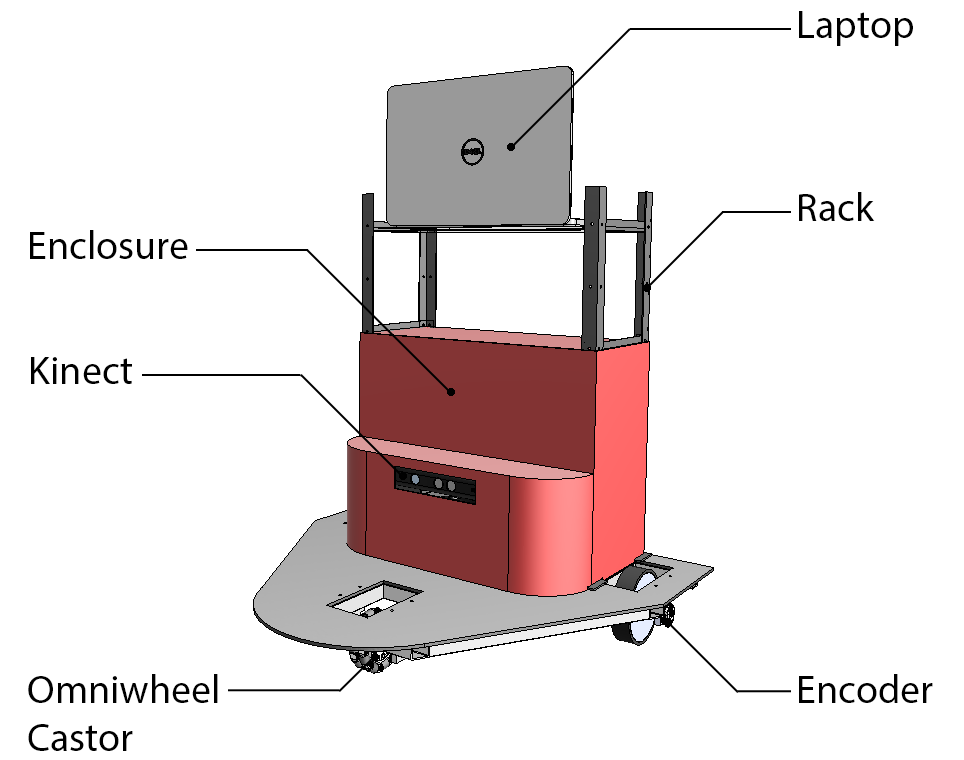
\includegraphics[scale=0.2]{Robot.png}
\caption{Robomuse 4.0 }
\end{figure}

\begin{figure}[H]
\centering
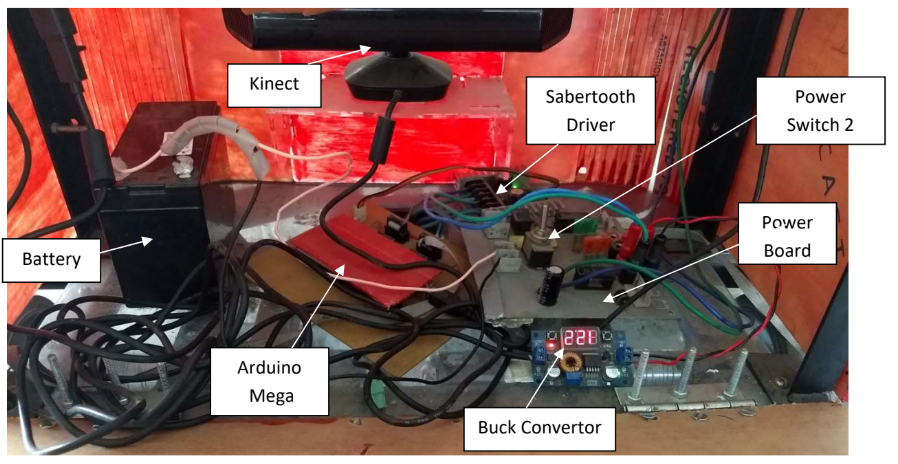
\includegraphics[scale=0.5]{RobotInterior.PNG}
\caption{Robot Circuit}
\end{figure}

\begin{figure}[H]
\centering
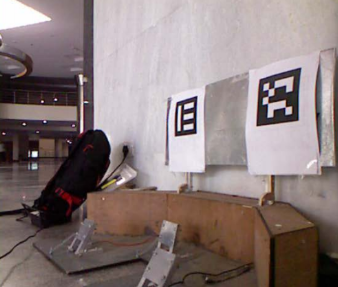
\includegraphics[scale=0.5]{ChargingStand.PNG}
\caption{Charging Dock}
\end{figure}

The robot is a differential drive robot with an omnidirectional wheel as a caster. It houses a Microsoft Kinect sensor for assimilating RGB-D images. It has an Arduino Controller and a laptop for processing. It is powered by Pb-Acid battery and a custom-build power supply circuit. It also features a charging circuit which allows for automatic docking and charging.

\newpage
\subsection{Odometry}
Odometry is the process of estimating the distance travelled and path travelled by the robot by mounting sensors on the shaft of the actuator. This can be used in the case of differential drive robots such as robomuse to estimate the x,y, yaw of the robot when it moves on a flat horizontal plane. However, this requires the assumption of pure rolling and no noise. SO we adopt a probabilistic version of this model.

% insert image of robot

In local frame of Robot
\begin{equation}v_{xr} = (\omega_{L} + \omega_{R})\frac{r}{2}\end{equation}
\begin{equation}
    v_{yr} = 0
\end{equation}
\begin{equation}
\omega_{zr} = (\omega_{R} - \omega_{L})\frac{r}{R}    
\end{equation}


% insert image of robot in xy plane

In global frame
\begin{equation}
    \begin{pmatrix}
    v_{x} \\
    v_{y} \\
    w_{z}
    \end{pmatrix}
     = 
    \begin{pmatrix}
    cos(\theta)  &&-sin(\theta)  &&0 \\
    sin(\theta)  &&cos(\theta)  &&0  \\
    0  &&0  &&1
    \end{pmatrix}
    \begin{pmatrix}
    v_{xr} \\
    v_{yr} \\
    w_{zr}
    \end{pmatrix}
\end{equation}
Taking multiplying by the inverse of the 3x3 matrix on both sides we get
\begin{equation}
    \begin{pmatrix}
    v_{x} \\
    v_{y} \\
    w_{z}
    \end{pmatrix}
    \begin{pmatrix}
    cos(\theta)  &&sin(\theta)  &&0 \\
    -sin(\theta)  &&cos(\theta)  &&0  \\
    0  &&0  &&1
    \end{pmatrix}
     = 
    \begin{pmatrix}
    v_{xr} \\
    v_{yr} \\
    w_{zr}
    \end{pmatrix}
\end{equation}
Summing $ v_{x}, v_{y} $ and $ \omega_{z}$ we can find the pose of the robot at any instant. This is called as odometry.

We can extend this model of odometry further by considering it in a probabilistic form.

\subsection{Mapping}
The process of creating a map of the environment using the depth image generated by the Kinect sensor is called mapping. The Robomuse uses an algorithm called RTAB (Real-Time Appearance Based) map to create a map of the surroundings. The mapping algorithm works by converting the depth image to a pseudo-2D laser scan of the surroundings so that the algorithm can determine the distance it is away from objects in its surroundings. RTAB map requires the tuning of parameters so that it can work and is present as a convenient ROS package.



\subsection{SLAM}
Simultaneous Localization and Mapping is a process where a robot maps an environment where it also uses the features of the environment to find its pose in it. It utilizes Extended Kalman filter and Particle filter to establish this. The data from the wheel odometry of the robot and the data obtained from the Kinect sensor are the input data to this method. It allows the robot to robustly estimate its pose with a probabilistic model rather than a deterministic model. The RTAB map package offers a SLAM extension, so the robot predicts its pose while mapping.


\subsection{Navigation}
The process of moving the robot autonomously from place to place in a known map is called navigation. The robot is equipped to navigate in the environment using a map of the environment and the wheel odometry data. When given a goal point, the robot plans a global path based on the map which it has. It also plans a local path based on the immediate sensor data it receives from the Kinect sensor. This ensures that the robot can perform static and dynamic obstacle avoidance. It uses A* search algorithm for global path planning and DWA planner for local motion planning. To interface all this, ROS provides a package called the navigation stack, which makes the development of a mobile robot a much faster job. The navigation stack requires parameters which have to be tuned based on the attributes of the robot currently working on, and once the parameters are set, the robot is ready to navigate in a map.


 
\subsection{ArUco markers}
ArUco marker is an augmented reality square marker which is surrounded by a black border and inside it contains a binary matrix which determines its unique identifier (id). The black border allows fast detection in the image in a lighter background, and the binary codification facilitates its identification, and it also uses various error correction coding methods for identification.

\begin{figure}[H]
\centering
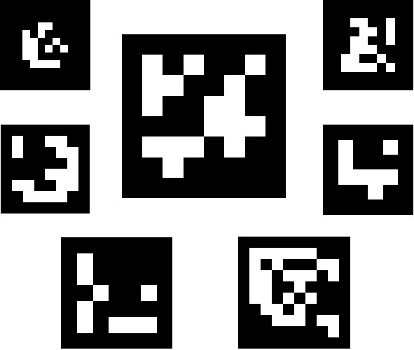
\includegraphics[scale=0.4]{markers.jpg}
\caption{ArUco Markers}
\end{figure}
 
 \subsection{Kidnapped robot problem}
The localization techniques developed can be distinguished according to the type of problem. Tracking or local techniques aim at compensating odometric errors occurring during robot navigation. However, they require that the initial location of the robot is known and they cannot recover if they lose track of the robot's existing position. Another set of approaches is global techniques. They are designed to estimate the position of the robot under any uncertainty. These techniques solve the wake-up robot problem, in that they can localize a robot without any prior knowledge about its position. Further, they can handle the kidnapped robot problem, in which a robot is carried to an arbitrary location during its operation. The wake-up problem is a particular case of the kidnapped robot problem in which the robot knows that it has been carried away. Global localization techniques are advanced than local ones. They can cope with situations in which the robot is likely to experience serious positioning errors.
 
 \subsection{PocketSphinx}
 CMU Sphinx is a package of speech recognition systems containing a series of speech recognizers and an acoustic model trainer. The speech decoders include acoustic models and sample applications. The available resources include software for acoustic model training, Language model compilation and a public domain pronunciation dictionary, cmudict.
PocketSphinx is a lightweight speech recognition engine, tuned explicitly for handheld and mobile devices. It is a part of the CMU Sphinx Open Source Toolkit For Speech Recognition.

\subsection{QT}
Qt is an open-source widget toolkit for creating graphical user interfaces as well as cross-platform applications. The interfaces are designed to run on various software and hardware platforms such as Linux, Windows, macOS, Android or embedded systems.

\newpage

\section{Marker Correction}

\subsection{Pose Estimation Algorithm}
\par The aruco\_ros package returns the pose of the marker with respect to the camera frame. By utilizing the ROS tf and tf2 packages, this can be converted to be in the form of X, Y, Z translations and Quaternion rotations.
\par \textbf{Quaternions for Rotations}
\par Unit quaternions, which are also known as versors, provide a convenient mathematical notation for representing orientations and rotations of objects in three dimensions. Compared to Euler angles they are simpler to compose and avoid the problem of gimbal lock. These are more compact, more numerically stable, and more efficient compared to rotation matrices. Quaternions have applications in computer graphics, computer vision, robotics, navigation, molecular dynamics, flight dynamics, orbital mechanics of satellites and crystallographic texture analysis.
\par Here, they are used for representing the rotation between the camera and the robot's base and the inverse.
\par When used to represent rotation, unit quaternions are also called rotation quaternions as they represent the three-dimensional rotation group. When used to represent an orientation (rotation relative to a reference coordinate system), they are called orientation quaternions or attitude quaternions.

\subsection{Pose embedded on the map}
\par To estimate the pose of the robot with respect to the marker we have to apply a frame transformation from the robot’s camera frame to the frame of the marker. This can be done by using the 6 DoF pose estimate yielded by the marker. The tf package of ROS allows us to perform this transformation with ease it obtains the rotation matrix for the marker and the translation. This is used to compute the location of the camera with respect to the marker.
\par The camera and the robot’s base link are connected via a static transformation. Once this transformation is done, the robot’s location with respect to marker can be estimated. 
\par First, let us consider mapping. We receive from the aruco\_ros package the transform of robot’s camera with respect to the marker. This can be viewed as robot’s base link with respect to marker whose transformation matrix we define as  $^{marker}_{base}T $. Now, we take inverse of this Transform
\begin{equation}
    ^{marker}_{base}T^{-1}
    =^{base}_{marker}T
\end{equation}


\par We use the odometry data to convert $^{marker}_{base}T $ to $^{map}_{marker}T $ where map is the frame from which we started to map from. If x,y,θ , are the x coordinate, y coordinate and θ is the angle robot makes with x-axis on xy plane, then
\begin{equation}
    ^{marker}_{base}T_{odometry} = 
    \begin{pmatrix}
    cos(\theta) && sin(\theta) &&0 &&x \\
    sin(\theta) && cos(\theta) &&0 &&y \\
    0 && 0&& 1&& 0 \\
    0 && 0&& 0&& 1
    \end{pmatrix}
    \end{equation}
Then,
\begin{equation}
    ^{map}_{marker}T = ^{map}_{base}T_{odometry}*^{base}_{marker}T
\end{equation}

\begin{figure}[H]
\centering
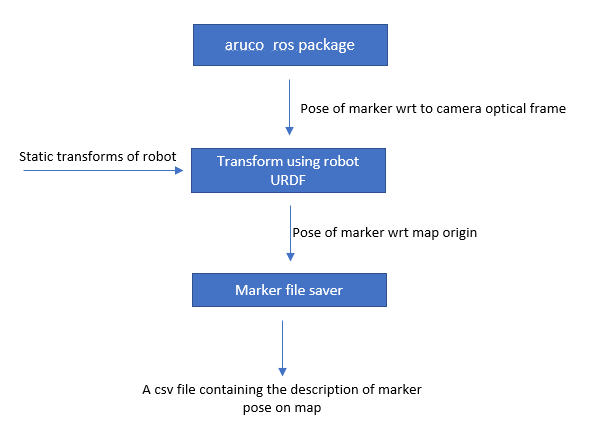
\includegraphics[scale=1]{1markermapping.PNG}
\caption{Mapping}
\end{figure}

\subsection{Loading markers during navigation}
While navigating autonomously using the navigation stack package the robot loads the already generated map while this is being loaded, the CSV file containing the marker pose with respect to the map can also be loaded. This can be generated as a tf frame. We also run the aruco\_ros package, which gets us the tf frames of the marker with respect to the camera on the robot. We can take the inverse of this transform and estimate the robot's pose with respect to the marker. Now we can utilize the existing data of where the marker is on the map and generate a pose estimate of the robot with only the saved marker data and estimated pose from the marker. This is a powerful tool. 

\subsection{Correction}
One application of the tool we discussed is as a correction procedure for correcting odometry of the robot as error accumulates over time. This can correctly estimate the robot's position and correct it. This can also be extended as a solution to the kidnapped robot problem. As a way to find the estimate of the pose of the robot when it is turned on in an unknown environment.
Now for correction given $ ^{map}_{marker}T $ Again we obtain $ ^{marker}_{base}T $ from aruco\_ros. Now we have to estimate $ ^{map}_{base}T $. To compute this all we need to do is:
\begin{equation}
    ^{map}_{base}T = ^{map}_{marker}T*^{marker}_{base}T
\end{equation}
\subsection{Filtering algorithm}
\par As expected from any direct sensor data, the pose data is noisy, and this is undesirable. We can implement a six-dimensional Kalman filter to filter out the noise and get a better pose estimate making the robot more reliable. The initial noise covariance matrix can be obtained from the initially obtained data during mapping the area this allows for faster convergence to correct value when estimating pose while navigating.

\begin{figure}[H]
\centering
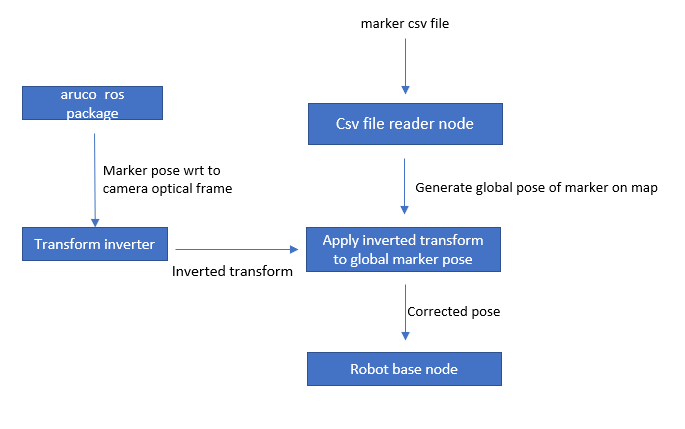
\includegraphics[scale=0.8]{1markernavig.PNG}
\caption{Navigation}
\end{figure}

\section{Multi Marker Extension}
\par The single marker-based pose correction can be extended to multiple markers by using simple adjustments to the filesystem and using the fact that each aruco marker possesses an ID. These IDs can be used to give each marker its location on the map uniquely. This is achieved through various things.

\subsection{Filesystem}
\par When the map is being created, a new directory is created by using the date and time of starting the program to preserve uniqueness. Inside this directory, several CSV files each named after the ID of the corresponding marker are generated and the poses of these with respect to the map are stored. This allows for correcting the Localization at many more locations and also allows kidnapped robot problem to be solved from broader area coverage.

\subsection{Dictionary style implementation}
\par The implementation of multiple markers needed the dynamic generation of tf frames when new markers were encountered. This was achieved by generating a new dictionary element whenever a new marker was encountered. The dictionary would start empty and fill as encountered, and when a marker is encountered, the dictionary is checked to ensure ID. The dictionary corresponded to the saving aspect within the file system so that the proper data is saved into the proper CSV file.

\subsection{Loading into navigation}
\par The file system is reaccessed based on the date and time given as parameters. Now a dictionary is created anew with data from the existing map markers present. Whenever a marker is encountered, the previously discussed algorithm estimates the pose of the robot. The presence of multiple markers introduces a challenge of choosing pose when multiple markers are in the visual frame. With previous data, we were able to estimate that markers which are closer by are more reliable for pose estimation, and the closer marker is used to estimate the pose. The additional advantage of putting multiple markers on the map allows generating waypoints to points based on the markers rather than defining ourselves by teleoperating the robot. It also allows the robot to increase its motion to a vast range, where corrections happen at regular intervals.
\newpage

\section{Improvement in Navigation}

\subsection{Navigation - Planner Improvement}

\subsubsection{Global Planner}
\par The global planner generates the trajectory from the source to the destination. The global-planner requires a map of the entire environment to calculate the best route.
\par There are three global planners - carrot planner, navfn and global planner. The carrot planner checks if the given goal is an obstacle, and picks an alternative goal close to the original one, by back-propagating along the vector between the robot and the goal point. Eventually, it passes this valid goal as a plan for the local planner or controller. Hence, this planner does not do any global path planning but is helpful when the robot has to move close to the given goal even if unreachable. The navfn planner uses Dijkstra's algorithm to find a global path with a minimum cost between the start point and endpoint. The global planner is built as a more flexible replacement of navfn with more options like support for A*, toggling quadratic approximation and toggling grid path.

\subsubsection{Local Planner}
\par The local planner creates new waypoints considering the dynamic obstacles and the vehicle constraints to transform the global path into suitable waypoints. So, the map is reduced to the surroundings of the vehicle and is updated as it is moving around to recalculate the path at a specific rate. It's not possible to use the whole map as the sensors cannot update the map in all regions, and a large number of cells would increase the cost of computation. Therefore, the local planning generates avoidance strategies for dynamic obstacles with the updated local map and the global waypoints and tries to match the trajectory as much as possible to the provided waypoints from the global planner. 
\par The most commonly used local planners for mobile robot applications are base\_local planner and DWA planner (dynamic window approach).
\par The basic idea of these local planner algorithms is as follows:
\begin{itemize}
    \item Sample the robot's control space (dx, dy, dtheta) discreetly. 
    \item For each sampled velocity, perform forward simulation from the robot's current state to predict what would happen if the sampled velocity were applied for some time. This may be done for the entire forward simulation or limited steps.
    \item Evaluate each trajectory resulting from the forward simulation, using a metric that incorporates characteristics such as proximity to obstacles, proximity to the goal, proximity to the global path, and speed. Discard illegal or impossible trajectories.
    \item Pick the highest-scoring trajectory and send the associated velocity to the mobile base.
    \item Rinse and repeat.
\end{itemize}

\textbf{Base local planner}\\ \\
The base\_local\_planner package provides a controller that drives a mobile base in the plane. This controller serves to connect the path planner to the robot. It is also known as Trajectory Rollout algorithm. Using a map, the planner creates a kinematic trajectory for the robot to get from a start to a goal location. Along the way, the planner creates, at least locally around the robot, a value function, represented as a grid map. Trajectory Rollout algorithm samples from the set of achievable velocities over the entire forward simulation period given the acceleration limits of the robot. This value function encodes the costs of traversing through the grid cells. The controller uses this value function to determine dx, dy, dtheta velocities to send to the robot.\\ \\
\textbf{DWA planner}\\ \\
The dwa\_local\_planner package provides a controller that drives a mobile base in the plane. This controller serves to connect the path planner to the robot. Using a map, the planner creates a kinematic trajectory for the robot to get from a start to a goal location. Along the way, the planner creates, at least locally around the robot, a value function, represented as a grid map. This algorithm samples from the set of achievable velocities over a small range, mostly one step forward simulation period, given the acceleration limits of the robot. This value function encodes the costs of traversing through the grid cells. The controller uses this value function to determine dx, dy, dtheta velocities to send to the robot.\\ \\
\textbf{Comparison}
\\ \\
DWA differs from base\_local planner in the way the control space of the robot is sampled. The base\_local planner samples from the set of achievable velocities over the entire forward simulation period given the acceleration limits of the robot, while DWA samples from the set of achievable velocities for just one simulation step given the acceleration limits of the robot. This means that DWA is a more efficient algorithm because it samples a smaller space. However, it may be outperformed by Trajectory Rollout for robots with low acceleration limits because DWA does not forward simulate constant accelerations.\\ \\

\textbf{Result}\\ \\
However, in practice, we found that DWA planner performed better in most of our test cases than base\_local\_planner. This is due to the reason that the robot moves in a closed environment. Hence there is no requirement of entire forward simulation, which thereby increases the efficiency of the computation. Moreover, the robot is designed for considerably high accelerations and rarely reaches extremely low speeds. With these considerations in mind, the DWA planner is implemented as the local planner.

\subsection{Recovery Behaviour}
Recovery behaviour is the response of the robot when it encounters an obstacle so close that the robot is stuck or is hindered of the forward motion. This case usually occurs when a dynamic obstacle suddenly appears on the map. The predefined recovery behaviour of the robot for this was to stop and make a complete revolution around itself to check for possible clearance for movement and then generate an alternative path. It is unnecessary to check for all possible clearances for any such cases. Hence, the recovery behaviour was changed. Now, the robot directly generates a path from its location to the goal if sufficient clearance is present between the robot and the obstacle. Otherwise, it makes a rotation until it finds enough clearance to cross the obstacle. This reduces the time of travel when such cases occur, which are highly predominant in a closed indoor environment.

\subsection{Artifacts in costmap - costmap clearing while stationary}
The term research artifacts refer to the uncontrolled and unintentional systematic biases, that can threaten the validity of one's conclusions. \\ \\
A problem with the cost map in 'RTAB' mapping is that when it detects an obstacle, it fixes it on the cost map permanently. So, even if the object is moved or removed, it still stays in the cost map. So, every time the program had to be restarted to clear the cost map of obstacles. To counter this, we made a recovery behaviour by resetting or clearing the cost map if the robot is stuck for a while, stopped or after reaching intermediate goals. This costmap clearing procedure is done by a separate node which runs independently it subscribes to the twist of the robot and goal status. Using this data, it calls the ros service to clear the costmap offered by the navigation stack.

\newpage

\section{Voice Control - PocketSphinx}

\subsection{Building a phonetic dictionary}
A phonetic dictionary provides a mapping of vocabulary words to sequences of phonemes. A dictionary file robomuse.dic was created with a set of vocabulary words for starting the robot, stopping, goal points, docking, etc.\\ \\
The recognizer searches for a word in both the dictionary and the language model and hence, for a word to be recognized, a language model file with all the words in the dictionary is created. Espeak is used to create the phonetic dictionary for the supported languages.

\subsection{Building a language model}
The language model is an essential component of the configuration which tells the sequences of words possible to be recognized by the decoder.\\ \\
Several models include keyword lists, grammar, statistical language models and phonetic language models. They have different capabilities and performance properties. 

\subsection{Keyword lists}
Pocketsphinx supports a keyword spotting mode whose advantage is that a threshold for each keyword can be specified so that keywords can be detected in continuous speech. Other modes try to detect the words from a grammar even if you used words which are not in the grammar.\\ \\
The threshold must be specified for every key phrase. For shorter key phrases smaller thresholds like 1e-1, for longer keyphrases, the threshold must be larger, up to 1e-50 are set. For very long keyphrases (larger than 10 syllables) it is split and spotted for parts separately. The threshold is tuned to balance between false alarms and missed detections.

\subsection{Grammar}
A grammar describes a simple type of language for command and control. They are created with the Java Speech Grammar Format (JSGF) with a file extension .gram or .jsgf.

\subsection{Language models}
Statistical language models contain probabilities of the words and word combinations. Those probabilities are estimated from sample data and automatically have some flexibility. Every combination from the vocabulary is possible, although the probability of each combination varies.

\subsection{Building a statistical language model - text preparation}
An extensive collection of clean texts is made with expanded abbreviations, numbers converted to words and non-word items are cleared. A reference text that is used to generate the language model is prepared with input in the form of normalized text files, with utterances delimited by <s> and </s> tags. A vocabulary file is then generated.

\subsection{Using the language model for control of Robomuse 4.0}
The language model created is then used for the control of Robomuse. The asr.launch file accesses the robomuse.dic dictionary file, robomuse.lm language model and asr.gram grammar file. The input, learning rule and hmm are set to default. The node asr\_test.py is created to handle the jspf grammar node. This node is responsible for the control of the robot by calling the required launch files under robomuse\_drivers. Another node send\_audio.py is created for publishing audio inputs.

\newpage

\section{QT - User Interface}

\subsection{Python scripts}
The python scripts are used for programming the effects of clicking buttons on the qt screen. The qt screen is generated from the design file which is of .ui form and can be generated form the qt designer software which allows drag and drop facilities to buttons and various other UI elements this allows for fast development. The python scripts inherently link to shell scripts which run other programs to run the robot.

\subsection{Shell scripts}
The shell scripts are used as timing elements and also used to call shell applications like espeak TTS service to allow the robot to say things. The essential function of the shell scripts is to time the launching of various nodes form the launch files. The timing facilitates the mitigation of errors while running and pipelines the entire process. The timing, however currently is done manually and times are measured for the proper launch of each file and time is set. However, this must be made such that it is synchronous in the future.

\subsection{Launch files}
Launch files have a collection of a logical cluster of nodes which have to be run together for a particular application. They also allow setting parameters for that particular applications so the same nodes can be run for different applications with different parameters. It allows for a greater extent of control and customization. This higher degree of customization and control can be leveraged for most of the operations. One example is the usage of the nodes of the RTAB map package where the nodes configured with different parameters can be used for the applications of mapping and then for navigation.

\begin{figure}[H]
\centering
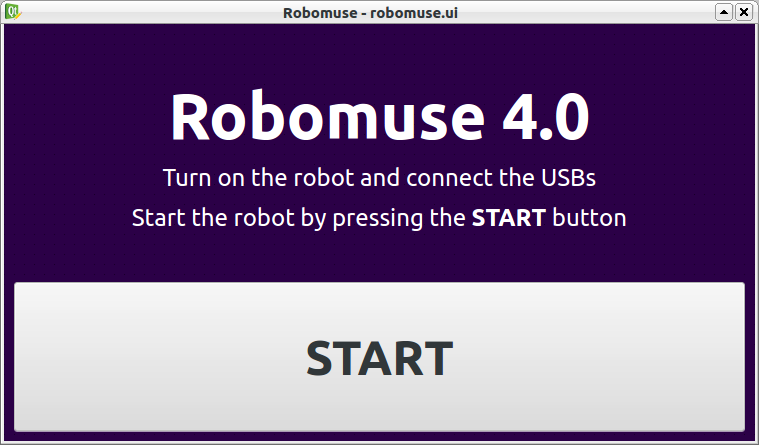
\includegraphics[scale=0.5]{Robomuse.png}
\caption{Start UI}
\end{figure}

\begin{figure}[H]
\centering
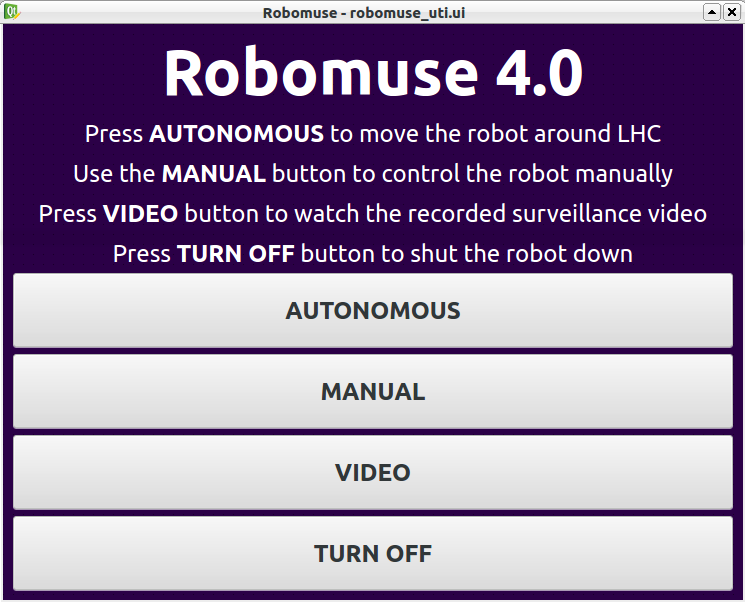
\includegraphics[scale=0.5]{Robomuse_uti.png}
\caption{Utilities UI}
\end{figure}

\begin{figure}[H]
\centering
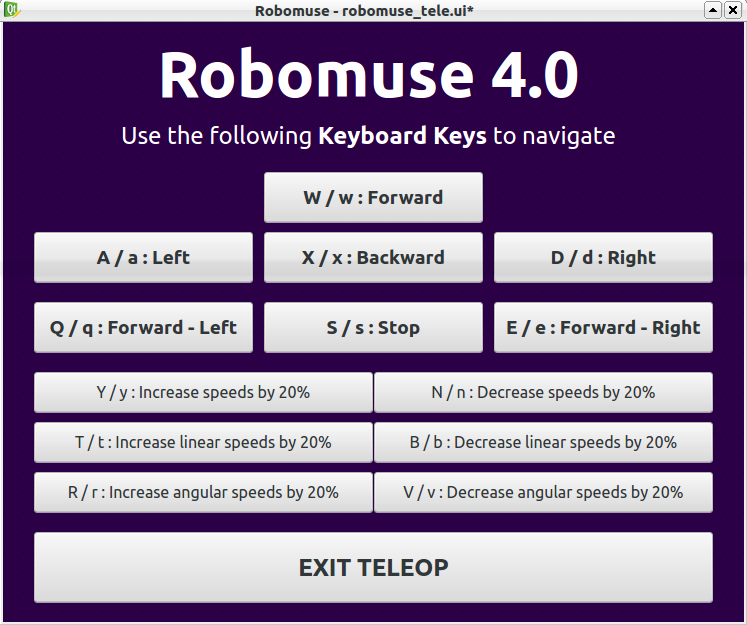
\includegraphics[scale=0.5]{Robomuse_tele.png}
\caption{Teleoperation UI}
\end{figure}

\subsection{Hierarchical structure and explanation of each node}
Robotstart- initial UI for starting the robot
	roscore - starts the rosmaster and ensures ros runs
startmenu.sh - a shell script to start the robot and run other shells 
	qtmenu node - (robomuse UI) launches the UI for the selection menu
		Nav.sh - runs shell scripts and launch files required to configure hardware
			Robomuse\_depthreg.launch - sets up the Kinect and Arduino
			Rtabnav.sh - sets up the slam
			Mbnav.sh - sets up the navigation stack
			Marknav.sh - sets up marker correction scripts
			Image\_view node - shows the camera feed
			Menu.sh - launches the menu
				Qtmenu\_uti node - robokmuse\_uti.ui
					Aroundlhc - node sends waypoints to the robot
					Teletoauto.sh - allows manual control scripts
						Teletoauto node - keyboard input
						Qtmenu\_tele node - robomuse\_tele.ui	
					Kill.sh - kills all proceses to stop the robot
\\ \\
This screen is launched when manual control is used. It is given for the guidance of the user about the control of the robot and teleoperation settings. 

\newpage

\section{Conclusion}
The work done over the summer saw the robot become more applicable in the real world. With more time and effort spent on the robot, the robustness of the system can be improved. Currently odometry errors tend to pile up in the robot and it eventually gets lost. To prevent this the $robot\_localization$ package can be implemented and an IMU can be used for sensor fusion of the odometry. Along with this the aruco markers can also act as fixed locations on a map with which the robot can correct it’s perceived  location on the map. With these done the robot will be made much more robust and many more applications can further be made.

\end{document}

%\section{Improvements in Existing Code}
% \label{sec:slam}
%\vspace{-0.2in} 
%\subsection{Creation of New Launch Files}
%Until summer of 2018 all code of RoboMuse was maintained by people who had exact knowledge about how the code worked. Hence for different applications, the same code was modified and used again. This modification of code may not be within the capabilities of a layman. Hence work was done to modularize the code by accurately pin-pointing what each ROS node does and separating them for their particular applications. For example, initially the $rtabmap$ node was publishing to the $rtabmap\_gridmap$ node and the $move\_base$ had been remapped to get input from it. This however is highly inconvenient as the map cannot be saved directly from $rtabmap\_gridmap$ and data had to be stored in a $rosbag$ and rerun. And to navigate on a map created with these launch files the remapping had to be manually removed before running $move\_base$ commands. To eliminate this problem completely, separate launch files with exact configurations for map-making, map-saving and navigating on a map were created.
%\\
%This led to the creation of the launch files $map\_rtab$ and $map\_move\_base$ for map-making and map-saving and $nav\_rtab$ and $nav\_move\_base$ for navigating on an existing map.

%\begin{figure}[h!]
%\centering
%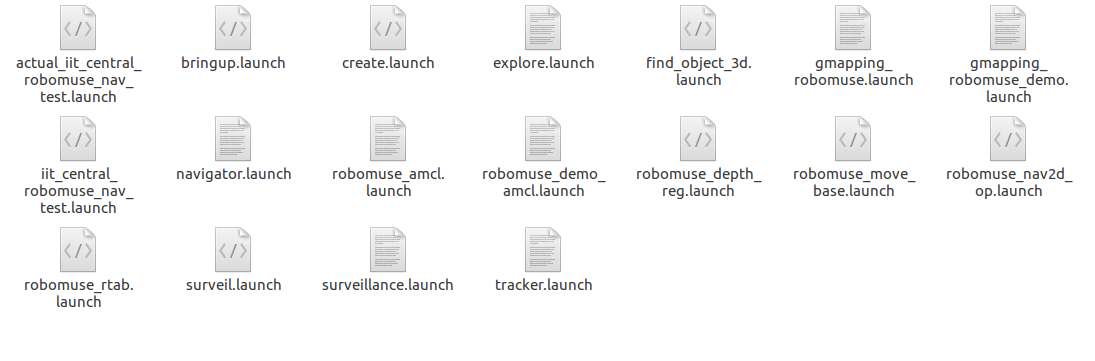
\includegraphics[width=0.7\textwidth]{beforelaunch.png}
%\caption{Package Before Launch files were added }
%\end{figure}

%\begin{figure}[h!]
%\centering
%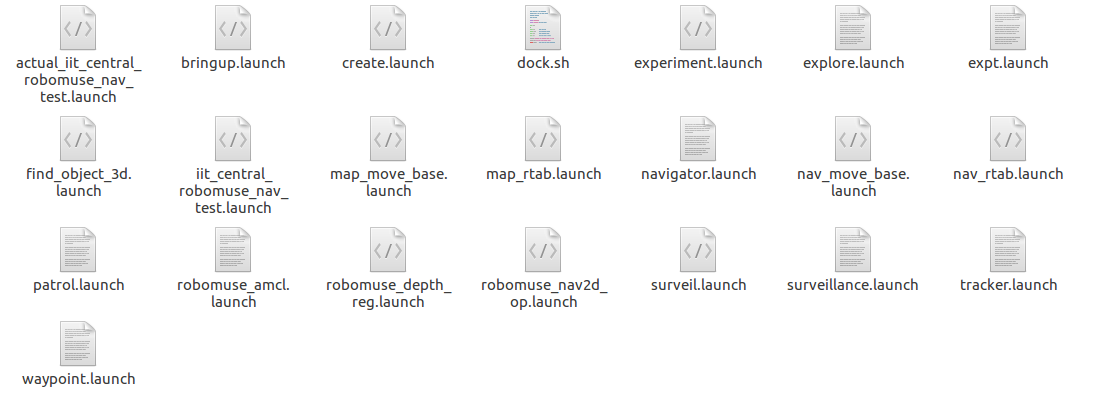
\includegraphics[width=0.7\textwidth]{afterlaunch.png}
%\caption{Package After Launch Files were added }
%\end{figure}

%\subsection{Teleoperation Using Android App}
%An inherent problem with the robot is that it has to be lifted to be moved from one place to another. Dragging the robot causes errors to occur with the encoders. Lifting the robot is generally a hard job because the robot weighs in excess of 20 Kg. To solve this issue, an already existing android app AIORemote (All In One Remote) was used to control the robot wirelessly. Code was written for teleoperation of the bot in python, a java program set up the server and the robot and the phone can be connected over a common Wi-Fi connection. A custom remote was created in the app which allows the RoboMuse to be controlled more effectively. This improved working conditions.

%\begin{figure}[h!]
%\centering
%\includegraphics[width=0.7\textwidth]{Screenshot_20180707-042824.png}
%\caption{Screenshot of RoboMuse remote }
%\end{figure}

%\subsection{Shell Scripts}
%Another problem plaguing RoboMuse was the need to run multiple commands in succession to get the robot to perform a function. To get around this issue various shell scripts were written to allow the robot to perform upon the running of 1 command whereas before the summer, 5 commands were required. This allowed the primary focus to application development. This also helps a layman work the robot better and also goes hand in hand towards the developing a GUI (Graphical User Interface) for the robot since modularity and grouping the commands are already created.
%\\
%Two types of shell scripts were created. Initially separately opening windows were made from the shell commands and ROS commands were run on each. This was not the right approach and hence a second more effective way of opening new tabs for each command was implemented.
%\\
%Another issue with running commands was ordering and timing them. This is crucial because some nodes require other nodes to be running to work. To solve this, all commands to be run to execute functions were studied and topologically sorted. Suitable delays were added and sync was achieved.
%\\
%Example shell scripts are as follows
%\\

%\begin{enumerate}
 %  \item ./map.sh
  % \begin{itemize}
   %  \item Running this command will allow you to map the environment the robot is in, using a single command. This is highly convenient for fast set up of the robot in a new location as it hides all the complexity associated with the programs running in the background.
   %\end{itemize}
   %\item ./setuptele
   %\begin{itemize}
%     \item This command starts the robot with the teleoperation capability. It also calls the java program that sets up a server and connects with the android AIORemote app and the custom remote of RoboMuse.
 %  \end{itemize}
  %\item ./nav
   %\begin{itemize}
    % \item This launches all the files needed for navigating on an existing map. It also starts the surveillance application built on the bot by default.
   %\end{itemize}
%\end{enumerate}

% ------------------Surveillance --------------------%
%\newpage
%\section{NavTest}
%\vspace{-0.2in}
%The robot was moved to Lecture Hall Complex and work was conducted there. Initially a CAD map of the environment was created and that was provided as map for the robot. Next, with the utility of the new $map\_rtab.launch$ and $map\_move\_base.launch$ files the centre of the Lecture Hall complex was mapped. This map was later fed to the robot’s navigation stack. Points were described within the map with the centre of the circle being the origin. A program was written to make the robot move to random points on this map and results were observed.
%\\
%The observations obtained from this were that the Adaptive Monte Carlo Localisation algorithm used during this process fails in some cases of symmetric environment and hence the node running the algorithm was not used; $rtabmap$ node alone was used to perform SLAM.

%\begin{figure}[h!]
%\centering
%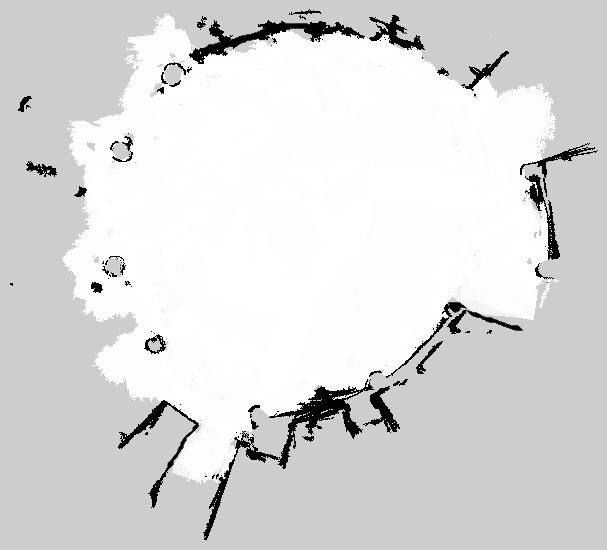
\includegraphics[width=0.7\textwidth]{lhc_IIT_central_Map2.jpg}
%\caption{Map of Lecture Hall complex generated by robot}
%\end{figure}

%\newpage

%\section{Charging Circuit}
%\vspace{-0.2in}
%\begin{figure}[h!]
%\centering
%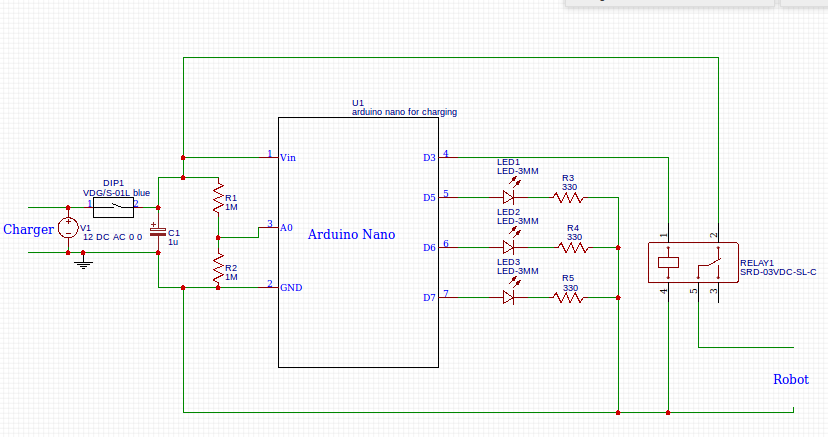
\includegraphics[width=0.7\textwidth]{charging_circuit.png}
%\caption{Schematic of Circuit}
%\end{figure}

%A charging circuit was developed for the battery of the robot so that the battery level could be monitored and the battery can be saved by cutting power during low charge. The working principle behind this is of the voltage divider circuit. Two resistors in series cause potential drops proportional to their resistance value and the current which flows through them. Hence when the battery has higher voltage the potential in the middle of the two resistors would be greater and charge is low vise versa.
%\\

%An Arduino Nano was used to observe this voltage through it’s onboard Analog to digital converter. Since the Arduino Nano works on 5V logic we can choose the resistors such that the potential at the resistor resistor junction is well placed in between the detection limits of the Arduino. Hence 5M ohm and 1M ohm resistors were chosen for this purpose. Now the potential at which the battery became incapable of powering the robot was experimentally found and and LEDs with suitable current limiting resistors in series were used to make them light up to different charge levels. Green meaning that the robot is charging. Blue meaning that the battery has sufficient charge and red meaning that the battery is low in charge.
%\\

%The Arduino also controlled a 5V relay which opens only when there is sufficient charge in the battery measured. Hence the charging circuit is a closed loop independent system to the robot\textsc{\char13}’s logic and motor control system.

%The schematic was made on the online free circuit designing application EasyEDA and the fabrication was done on a perf-board with through hole components.
%\newpage

%\begin{figure}[h!]
%\centering
%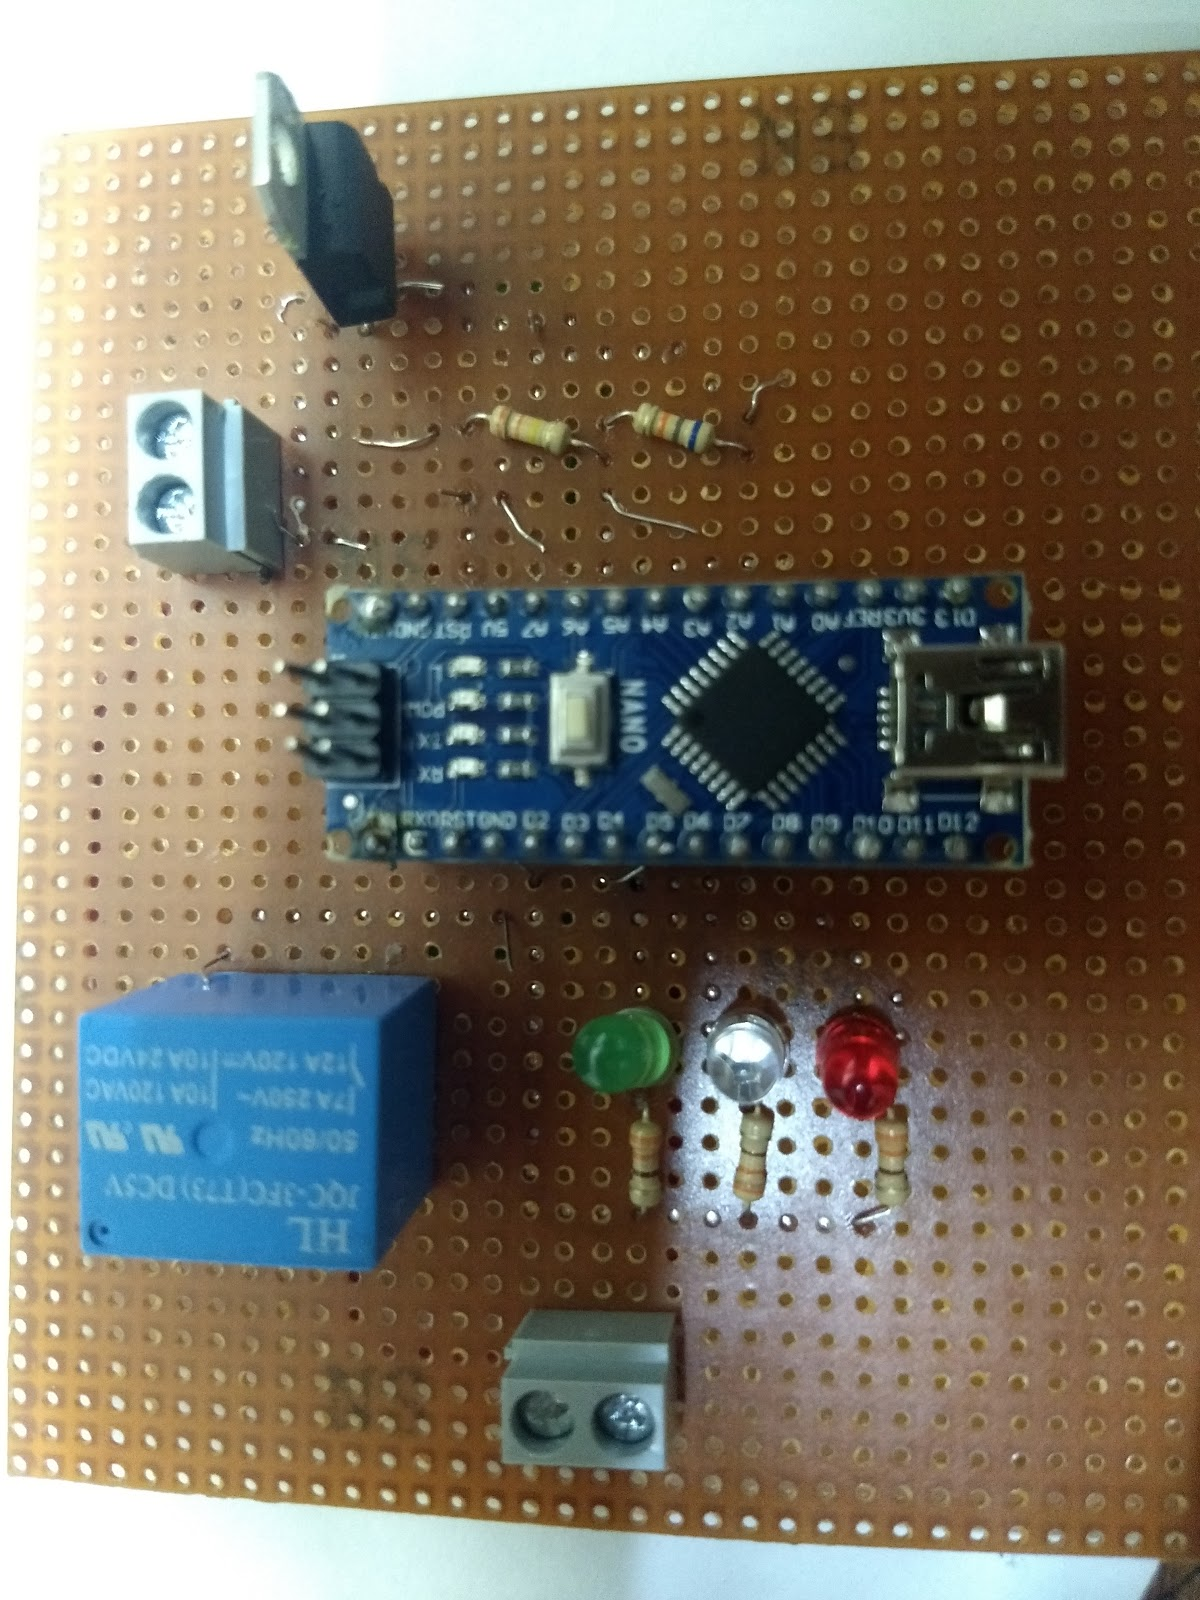
\includegraphics[width=0.7\textwidth]{cirtop.jpg}
%\caption{Image of the Circuit}
%\end{figure}

%\newpage

%\section{Docking using QR Code}
%\vspace{-0.2in}

%The robot requires charging at appropriate intervals and if the charging can be done by the robot autonomously it eases the work of the user. The previous docking port was refurbished into working condition and the mechanism of docking was improved. The leads from the dock directly fit into the charging circuit allowing for autonomous charging. Work was done to make a robust algorithm that made the robot dock in the port reliably. The existing algorithm was replaced by an algorithm that first placed the robot in clear view of the dock. Then the location of the dock with respect to the $base\_link$ was obtained and saved for use. Then phase 2 of the docking algorithm is run. This triggers a P controller based on the error between the differences of the distances from the two QR codes (Quick Response Code). The robot moves forward as it adjusts it’s pose.

%\begin{figure}[h!]
%\centering
%\includegraphics[width=0.7\textwidth]{illus.png}
%\caption{Illustration of Docking}
%\end{figure}

%\newpage

%The identification of the QR codes is done through the find\_object\_2d package and through the find\_object\_3d node. The SIFT (Scale Invariant Feature Transform) algorithm is used to feature match an existing image of the QR code to the live feed.

%\begin{figure}[h!]
%\centering
%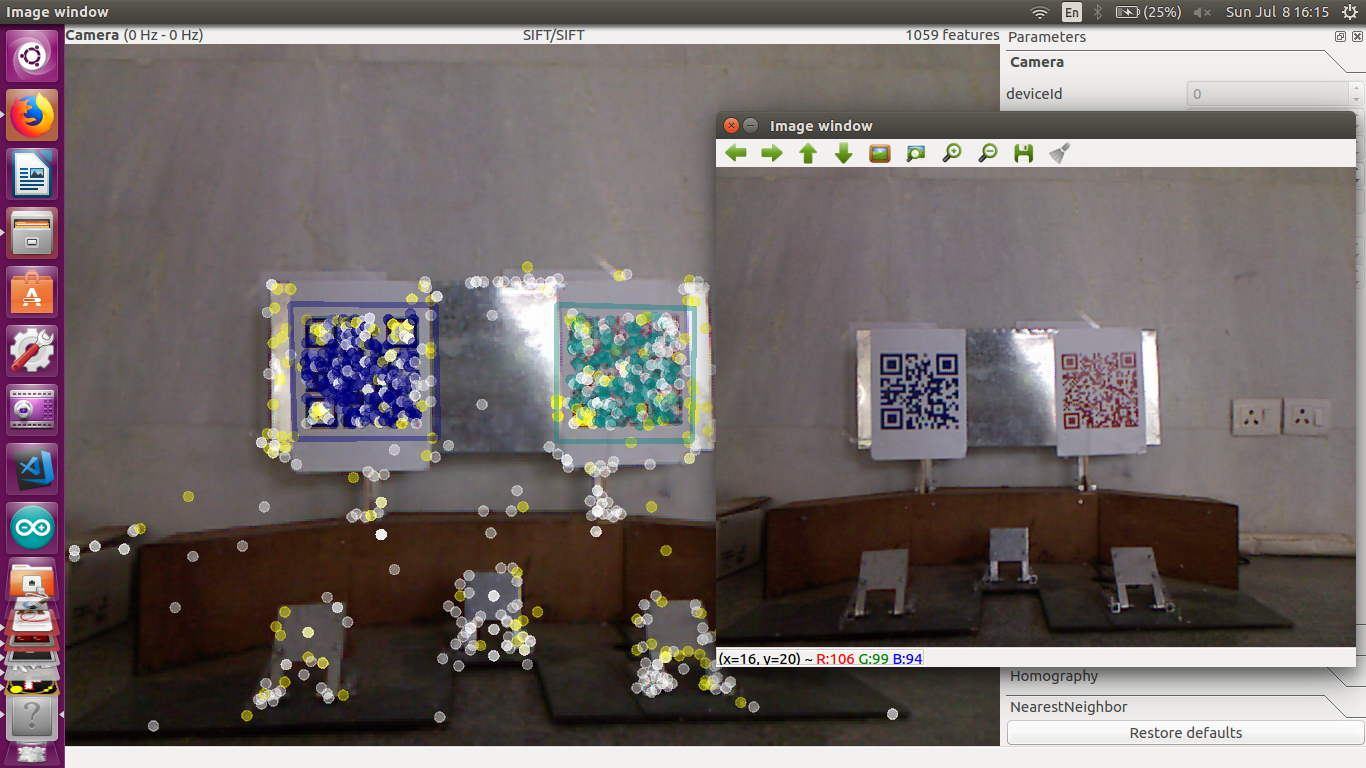
\includegraphics[width=0.7\textwidth]{qr_capture.png}
%\caption{Detection of QR using find\_object\_3d node}
%\end{figure}

%\newpage

%\section{Aruco Markers}
%\vspace{-0.2in}

%Inspired from Augmented Reality the concept of Aruco markers was used to dock the robot.
%\\

%\begin{figure}[h!]
%\centering
%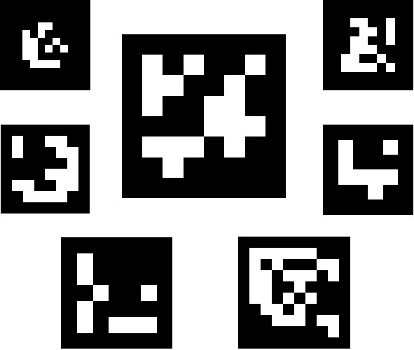
\includegraphics[width=0.7\textwidth]{markers.jpg}
%\caption{Some examples of Aruco markers}
%\end{figure}

%This method is much more efficient because these markers utilize their unique geometry and the binary codes embedded in them to locate them rather than blind feature recognition which is much more resource hungry. The effectiveness of these markers comes from the fact that the vision algorithm can very accurately estimate both location and pose of the marker even when it is tilted at various angles. This is not the case when it comes to feature recognition used in QR codes.

%\begin{figure}[h!]
%\centering
%\includegraphics[width=0.7\textwidth]{aruccap1.png}
%\includegraphics[width=0.7\textwidth]{aruccap2.png}
%\caption{Detection of Aruco Markers with pose}
%\end{figure}

%\newpage

%\section{Comparison of Docking}
%\vspace{-0.2in}

%The same movement algorithm used for docking using QR code is used for the Aruco markers for fair comparison between the two markers.

%\subsection{Aruco Markers vs QR codes in terms of Detection Range}
%The difference in maximum distance at which the markers are recognized by the robot is crucial for docking. Some experiments were performed to accurately determine this. The robot was placed 4m directly in front of the dock facing it and was made to move very slowly by publishing /robomuse/cmd\_vel. A program was written to print the distance from the dock from robot if detected and the following results were obtained.



%\begin{table}[h!]
%\centering
%\begin{tabular}{ |p{3cm}|p{3cm}|  }
% \hline
 %S.No. & Distance in m \\
 %\hline
 %1   & 2.50\\
 %2   &  2.52\\
 %3   & 2.61\\
 %4   & 2.59\\
 %5   &   2.50\\
 %\hline
 %Average& 2.54\\
 %\hline
%\end{tabular}
%\caption{Distance of Detection For QR codes}
%\end{table}

%\begin{table}[h!]
%\centering
%\begin{tabular}{ |p{3cm}|p{3cm}|  }
% \hline
 %S.No. & Distance in m \\
 %\hline
 %1   & 2.52\\
 %2   &  2.63\\
 %3   & 2.72\\
 %4   & 2.72\\
 %5   &   2.63\\
 %\hline
 %Average& 2.64\\
 %\hline
%\end{tabular}
%\caption{Distance of Detection For Aruco Markers}
%\end{table}

%The study concludes that Aruco Markers provide a greater detection range by 10cm.
%\newpage
%\subsection{Aruco Markers vs QR codes in terms of Angle of Detection}
%Even though the current algorithm takes away the need to have large angular detection. It is a good indicator of how robust the markers are.

%\begin{figure}[h!]
%\centering
%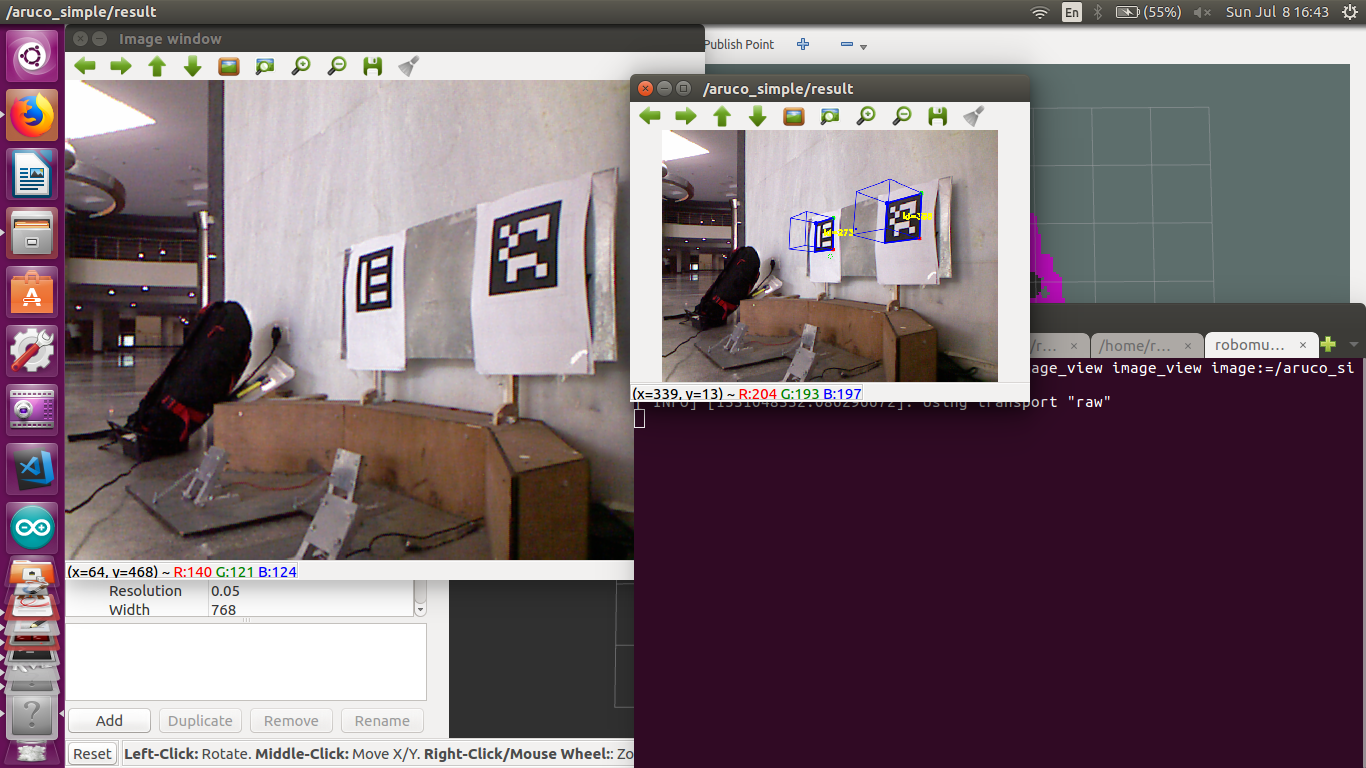
\includegraphics[width=0.7\textwidth]{detection_max_angle.png}
%\caption{Illustration of detection of both Aruco markers at a large angle}
%\end{figure}
%\begin{figure}[h!]
%\centering
%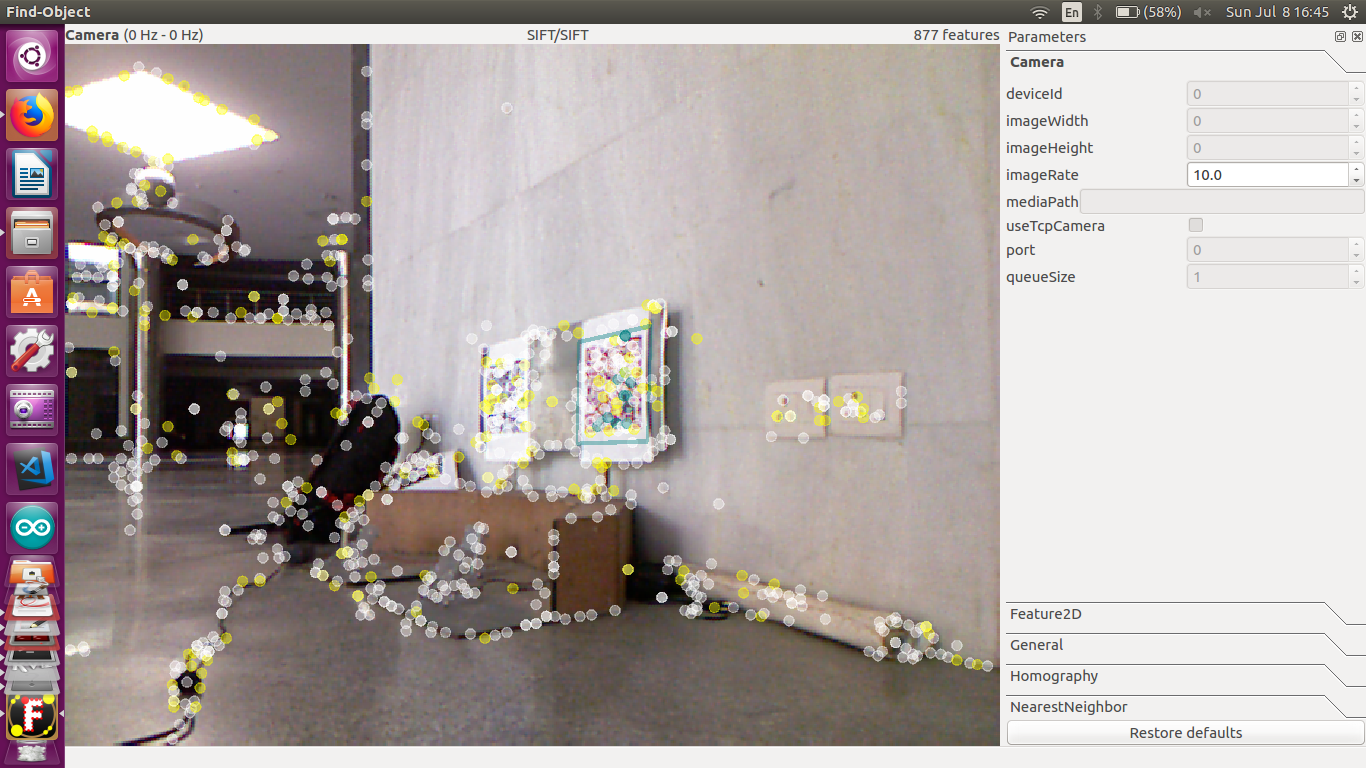
\includegraphics[width=0.7\textwidth]{qrnotdetec.png}
%\caption{Illustration of failure to detect farther QR code at a large angle}
%\end{figure}

%By viewing these two images the conclusion that Aruco Markers are better at angular detection can be made. The detection of Aruco Markers is detected up to 60 degrees and beyond this the performance decreases.

%\newpage

%\subsection{Aruco Markers vs QR codes in terms of Frame Rate}
%For any Computer Vision based application the Frame Rate of images is the most important indicator of efficiency of the algorithm. Higher the frame rate, more efficient the algorithm. Since both QR code detection using SIFT and Aruco marker detection using contours are both Computer Vision applications,  the analysis of frame rate is crucial in determining the better algorithm.\\
%To do this the frame rates were measured by using the $rqt\_tf\_tree$ publish frequency. Since this frequency is the frame rate of the images.

%\begin{figure}[h!]
%\centering
%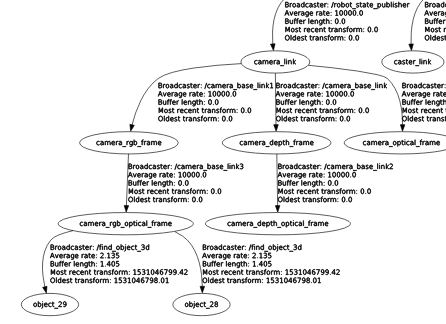
\includegraphics[width=0.7\textwidth]{lower_frame_rate.png}
%\caption{Illustration of the extremely slow rate of publication of QR code}
%\end{figure}

%\begin{figure}[h!]
%\centering
%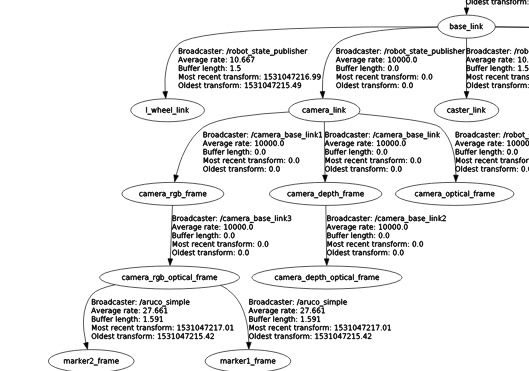
\includegraphics[width=0.7\textwidth]{arucorate.png}
%\caption{Illustration of the very good rate of publication of Aruco Markers}
%\end{figure}

%\newpage

%From the image we can see that the Aruco marker frame rate is about 27 hertz and frame rate of QR code is 2 hertz. This frame rate can be compared to the native image publish rate of 30 hertz of the kinect and we can see clearly the Aruco marker based algorithm is the better one.

%\newpage

%\section{Surveillance Application}
%The previously developed surveillance application was made more robust by adding way-point following and obstacle avoidance to the robot. The earlier program provided $cmd\_vel$ for a particular time; now it it done through providing $move\_base$ goals which allows it to avoid obstacles. An area was selected for the robot and was mapped similar to the NavTest. Way-points were found on the map and the robot was made to move to these way points in a closed loop. As it does so all the video data is stored. Also an interrupt trigger was set up. Once this trigger is activated the robot automatically performs the docking algorithm. This can be used by security personnel for surveillance and that was the inspiration behind this application.

%\begin{figure}[h!]
%\centering
%\includegraphics[width=0.7\textwidth]{surveil.png}
%\caption{Map of the area under surveillance}
%\end{figure}
%\newpage




